\documentclass[12pt]{beamer}
\usetheme{Warsaw}
\usepackage[utf8]{inputenc}
\usepackage{amsmath}
\usepackage{amsfonts}
\usepackage{amssymb}
\usepackage{graphicx}
\usepackage[font=Times,timeinterval=1,timeduration=2.0,timedeath=0,fillcolorwarningsecond=white!60!yellow,timewarningfirst=50,timewarningsecond=80,resetatpages=2]{tdclock}
\usepackage{tabularx}
\usepackage{array}
\usepackage{multicol}
\usepackage{longtable}
\usepackage{xcolor}
\usepackage{textcomp, gensymb}
\usepackage{pgfplots}
\usepackage[makeroom]{cancel}

\graphicspath{ {./references/} }
\pgfplotsset{
	soldot/.style={color=black,only marks,mark=*},
	holdot/.style={color=black,fill=white,only marks,mark=*},
	compat=1.12
}
\newcolumntype{Y}{>{\centering\arraybackslash}X}
\makeatletter
\def\@listii{\leftmargin\leftmarginii
			  \topsep    2ex
			  \parsep    0\p@   \@plus\p@
			  \itemsep   \parsep}
\makeatother
\newcommand\at[2]{\left.#1\right|_{#2}}

\begin{document}
\begin{frame}
	\frametitle{Bellwork 12/12}
	\initclock

	\vfill
	\large
	The following data describes the motion of a particle:
	\begin{center}
		\[a(t)=3\cos(t)-2\sin(t)\text{; }s(0)=0\text{; }v(0)=4\]
	\end{center}
	\vfill
	\vfill
	Find the particle's position function $s(t)$.
	\vfill
	\vfill
	\vfill
	\vfill

	\small
	\crono
	\resetcrono{\beamerbutton{reset}}
\end{frame}
\begin{frame}
	\frametitle{Bellwork 12/12 - Solution}

	\small
	\begin{align*}
		\int_{0}^{t}a(t)\,dt & \implies v(t)-v(0)=3\sin(t)+2\cos(t) \\
		& \implies v(t)=3\sin(t)+2\cos(t)+4
	\end{align*}
	\begin{align*}
		\int_{0}^{t}v(t)\,dt & \implies s(t)-s(0)=-3\cos(t)+2\sin(t)+4t \\
		& \implies \boxed{s(t)=-3\cos(t)+2\sin(t)+4t}
	\end{align*}
\end{frame}
\begin{frame}
	\frametitle{Exercise 1}

	\large
	Find the area under the piecewise curve below:
	\vfill
	\begin{center}
		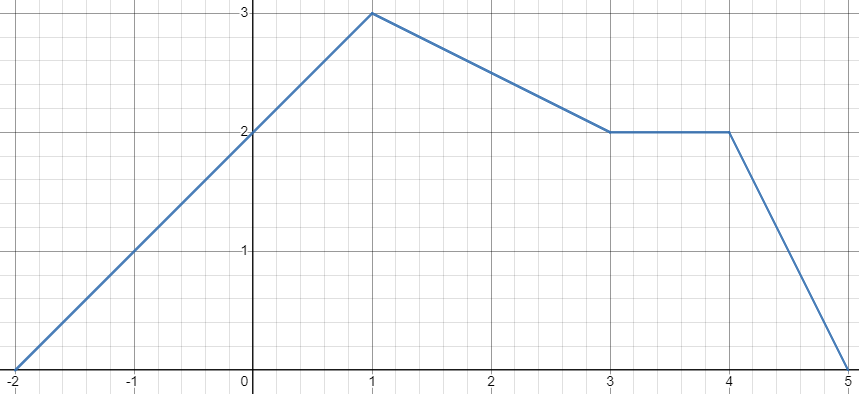
\includegraphics[scale=0.45]{exercise_1_graph.png}
	\end{center}
\end{frame}
\begin{frame}
	\frametitle{Exercise 1 - Solution}

	\large
	\begin{center}
		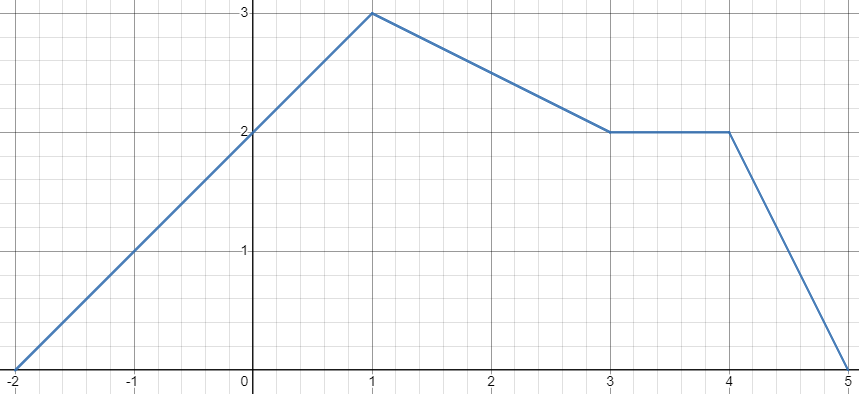
\includegraphics[scale=0.45]{exercise_1_graph.png} % *: The regional areas are to be written-in on the regions.
	\end{center}
	\vfill
	\[2+8+1+\frac{3}{2}=\boxed{11+\frac{3}{2}}\]
\end{frame}
\end{document}